Para el desarrollo de cada Sprint, se utiliza una aplicación gratuita y Open Source llamada Taiga, la cual es una plataforma de gestión de proyectos para diseñadores ágiles.

Para comenzar a utilizar esta plataforma se deben registrar las historias de usuarios con su respectiva prioridad (etapa conocida como Product Backlog). Una vez realizado lo anterior, se proceden a crear los Sprints y por último se añaden las historias de usuarios a cada uno de estos tal como se muestra en la \textbf{Figura~\ref{fig: SprintBacklog}} y en caso de ser necesario, una historia del Product Backlog puede ser subdividad para lograr un mejor enfoque y claridad en el desarrollo.

\begin{figure}[h!]
    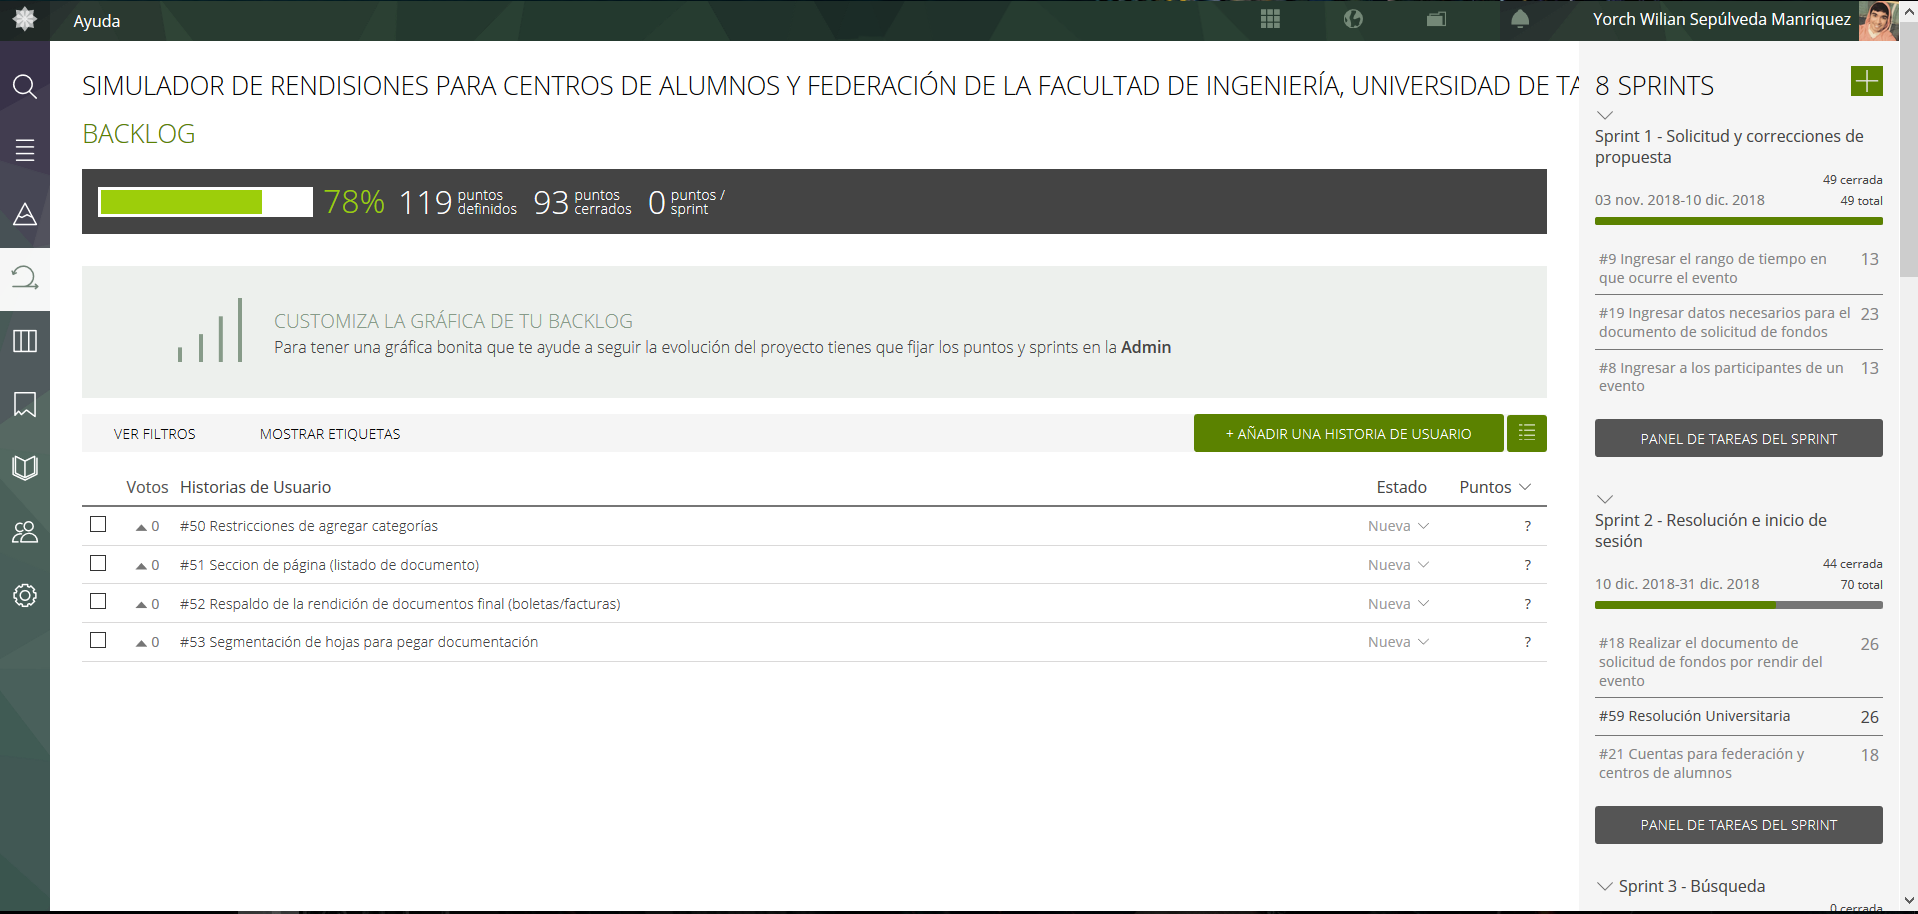
\includegraphics[width=\textwidth]{Imagenes/SprintBacklog.png}
    \caption{\label{fig: SprintBacklog} Sprint Backlog.}
\end{figure}

Dentro de cada Sprint hay un Kanban, el cual ayuda a organizar el desarrollo de cada historia de usuario realizada en el Sprint Backlog, en donde divide el trabajo en pequeñas tarjetas o tickets.

Dado lo anterior es que se divide el proceso de trabajo en cinco columnas como se muestra en la \textbf{Figura~\ref{fig: kanbanSprint}}, en donde se encuentra:

\begin{itemize}
    \item   \begin{description}
                \item[Nueva:] Se ingresan pequeñas tarjetas o ticket de trabajo que ayudan a realizar el cumplimiento de la historia de usuario.
            \end{description}

    \item   \begin{description}
                \item[En curso:] sección en donde se encuentran las tareas que se están realizando.
            \end{description}

    \item   \begin{description}
                \item[Lista para Testear:] columna en la que se encuentran las tareas terminadas y en proceso de aceptación.
            \end{description}

    \item   \begin{description}
                \item[Cerrada:] área en donde se encuentran las tareas que han sido finalizadas y aceptadas.
            \end{description}
    
    \item   \begin{description}
                \item[Necesita Información:] sección en donde se encuentran las tareas que no han logrado culminarse debido a que falta información para su realización.
            \end{description}
\end{itemize}

\begin{figure}[h!]
    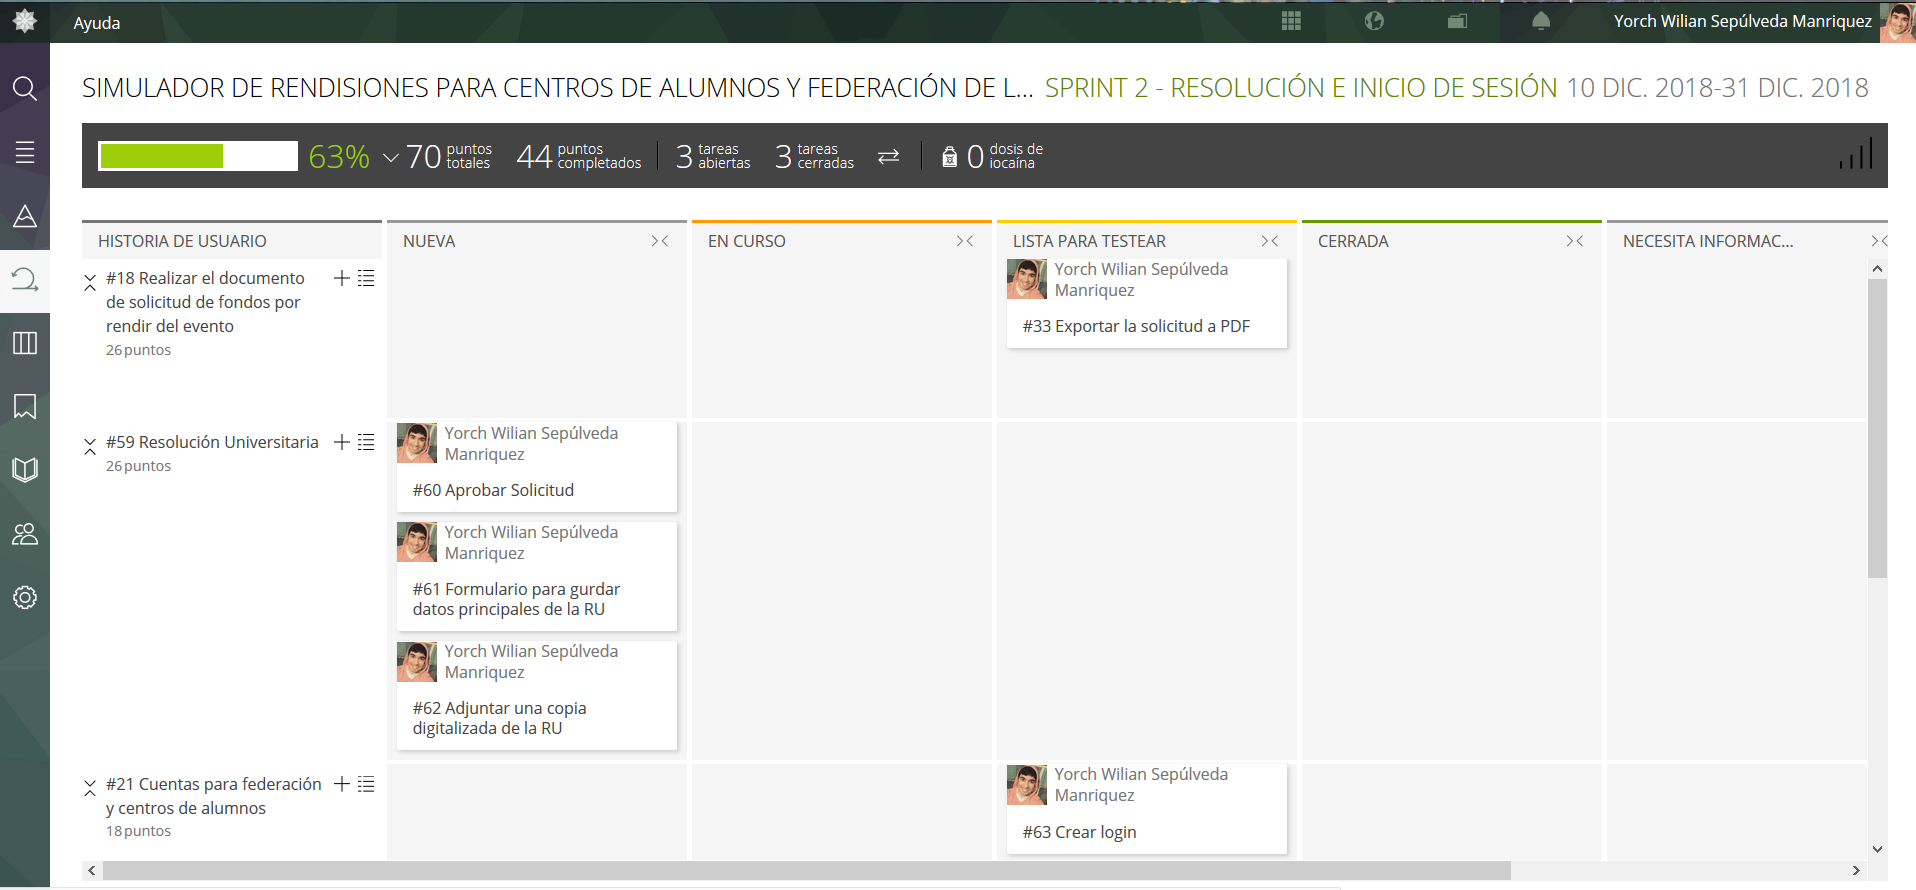
\includegraphics[width=\textwidth]{Imagenes/Kanban.png}
    \caption{\label{fig: kanbanSprint} Proceso de trabajo de un Sprint.}
\end{figure}

Para el diseño de base de datos se usa una aplicación llamada draw.io~\cite{20} para diseñar el diagrama Entidad/Relación (E/R). Luego de diseñar el diagrama E/R, se procede a crear el modelo relacional y para esto se utiliza StarUML, que permite la creación de estas tablas de forma gráfica y exportar todo esto a código, el cual es importado en MySQL que es donde está alojada la base de datos. StarUML no sólo se utiliza para diseñar la base de datos, sino que también para la creación de la arquitectura lógica y el diagrama de clases. 

En cuanto al desarrollo de la aplicación se utiliza el framework ASP.NET Core (ver \textbf{Sección \ref{sec:Tecnologias}}). Esta tecnología utiliza HTML-Razor para estructurar las vistas que el usuario puede acceder y a su vez, este último utiliza CSS el cual describe cómo es la presentación de la vista. Además, con la ayuda de JavaScript hace que la aplicación sea dinámica. También se utiliza C\# debido a que forma parte de la plataforma dotNET. Este ayuda a generar el programa sobre la plataforma. 

 Por otra parte, en primera instancia se utiliza el IDE Visual Studio para la creación del proyecto. Pero a lo largo del desarrollo, se cambió de IDE a VSCode, ya que había que utilizar una librería para la creación de archivos PDF que era incompatible con Visual Studio.

Por último, se utiliza Bizzagi Modeler para la creación de diagramas de flujo que permiten comprender el proceso de solicitud de fondos por rendir tanto para Federación como para Centros de Alumnos.